\documentclass{beamer} %[handout]
\usetheme{CambridgeUS}
\usecolortheme{whale}
\usepackage{color}
\usepackage{xcolor}
\usepackage[makeroom]{cancel}
\usepackage{graphicx} 
\setbeamercolor{frametitle}{fg=black}
\usepackage{mathtools}
\usepackage{amssymb}
\usepackage{amsmath}
\usepackage{amsthm}
\usepackage{graphicx}
\usepackage{fancyvrb}
\usepackage{listings}
\usepackage{tikz}
\usepackage[utf8]{inputenc}

\usetikzlibrary{shapes}

\usetikzlibrary{decorations.text}

\lstset{frame=tb,
  language=R,
  aboveskip=3mm,
  belowskip=3mm,
  showstringspaces=false,
  columns=flexible,
  basicstyle={\tiny\ttfamily},
  numbers=none,
  numberstyle=\tiny\color{gray},
%  keywordstyle=\color{blue},
%  identifierstyle=\color{yellow},
  breaklines=true,
    literate={->}{$\rightarrow$}{2}
           {°}{$\epsilon$}{1},
  breakatwhitespace=true
  tabsize=3
}

\usetikzlibrary{arrows,positioning} 
\tikzset{
    %Define standard arrow tip
    >=stealth',
    %Define style for boxes
    punkt/.style={
           rectangle,
           rounded corners,
           draw=black, very thick,
           text width=6.5em,
           minimum height=2em,
           text centered},
    % Define arrow style
    pil/.style={
           ->,
           thick,
           shorten <=2pt,
           shorten >=2pt,}
}

\makeatletter
\def\th@mystyle{%
    \normalfont % body font
    \setbeamercolor{block title example}{bg=orange,fg=white}
    \setbeamercolor{block body example}{bg=orange!20,fg=black}
    \def\inserttheoremblockenv{exampleblock}
  }
\makeatother
\theoremstyle{mystyle}
\newtheorem*{remark}{Example}

\makeatletter
\def\th@mystylet{%
    \normalfont % body font
    \setbeamercolor{block title example}{bg=purple,fg=white}
    \setbeamercolor{block body example}{bg=purple!20,fg=black}
    \def\inserttheoremblockenv{exampleblock}
  }
\makeatother
\theoremstyle{mystylet}
\newtheorem*{analysis}{Example}

\date{}
\author[Bayesian statistics]{Erik \v{S}trumbelj\\2019}

\linespread{1.2}
\renewcommand{\thefootnote}{\roman{footnote}}
%\setbeameroption{show notes}

\title[Stan]{Probabilistic programming with Stan}

\begin{document}

\begin{frame}

\centering
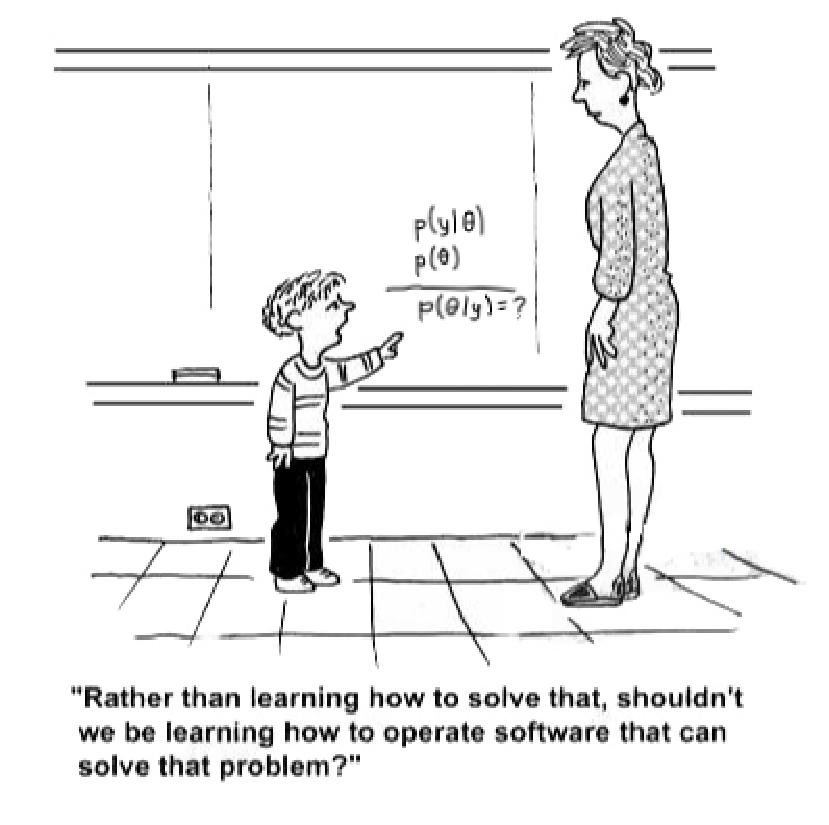
\includegraphics[width=0.60\linewidth]{../LectureAssets/L03/Lecture03Cartoon}
\end{frame}

\begin{frame}
Bayesian statistics
\titlepage
\end{frame}

\begin{frame}{Stan software for Bayesian inference}

\bigskip

\begin{center}

\includegraphics[scale=0.3]{../LectureAssets/L03/stan_logo}
\end{center}

\bigskip

\bigskip

\textbf{Stan is composed of}

\begin{enumerate}
\item a probabilistic programming language,
\item a math and auto-differentiation library,
\item MCMC sampling-based inference algorithm.
\end{enumerate}

\bigskip

We describe our model in Stan and Stan does the computation!

\bigskip

\bigskip

\end{frame}


\begin{frame}{Stan}

\bigskip

\begin{center}\url{http://mc-stan.org/}\end{center}

\bigskip

\textbf{Summary:}

\begin{itemize}
\item Software tool for Bayesian statistics,
\item inference based on Hamiltonian Monte Carlo,
\item written in C++ (Win, Mac, Linux),
\item interfaces in R, Python, MATLAB, Julia, Stata, Mathematica, Scala...
\item open source (BSD, PLv3),
\item great documentation (manual, studies; see website),
\item constant development, active community (\url{discourse.mc-stan.org/}).
\end{itemize}

\bigskip

\end{frame}

\begin{frame}{Stan - other functionality}

\smallskip

\textbf{Several inference algorithms:}

\begin{itemize}
\item NUTS (No-U-Turn Sampler, variant of HMC). 
\item HMC.
\item Structural approximation (Variational Inference, Laplace approximation).
\item Classic gradient-based optimization (L-BFGS, BFGS).
\end{itemize}

\bigskip

\textbf{User-friendly interfaces and tools in R:}

\begin{itemize}
\item \texttt{RStanArm}: Bayesian equivalents of \texttt{lm()}, \texttt{glm()},\texttt{polr()}...
\item \texttt{ShinyStan}: Interactive summary of results and MCMC diagnostics.
\item \texttt{loo}: Model evaluation and comparison.
\end{itemize}


\end{frame}

\begin{frame}{Further reading}

The Stan Language Reference manual contains a lot of valuable information both on how to use Stan and on standard statistical models written in Stan.

\bigskip

Stan/rstan reference sheet: \url{https://github.com/sieste/Stan_cheatsheet}

\bigskip

A good book on Bayesian statistics aimed at practitioners of statistics and not heavy on the math:

\begin{scriptsize}
\begin{itemize}
\item[] Kruschke, John. Doing Bayesian data analysis: A tutorial with R, JAGS, and Stan. Academic Press, 2014.
\end{itemize}
\end{scriptsize}
\end{frame}


\end{document}
